\section{PartTwoOptInit Class Reference}
\label{class_part_two_opt_init}\index{PartTwoOptInit@{PartTwoOptInit}}
It sets the first couple of edges.  


{\tt \#include $<$part\_\-two\_\-opt\_\-init.h$>$}

Inheritance diagram for PartTwoOptInit::\begin{figure}[H]
\begin{center}
\leavevmode
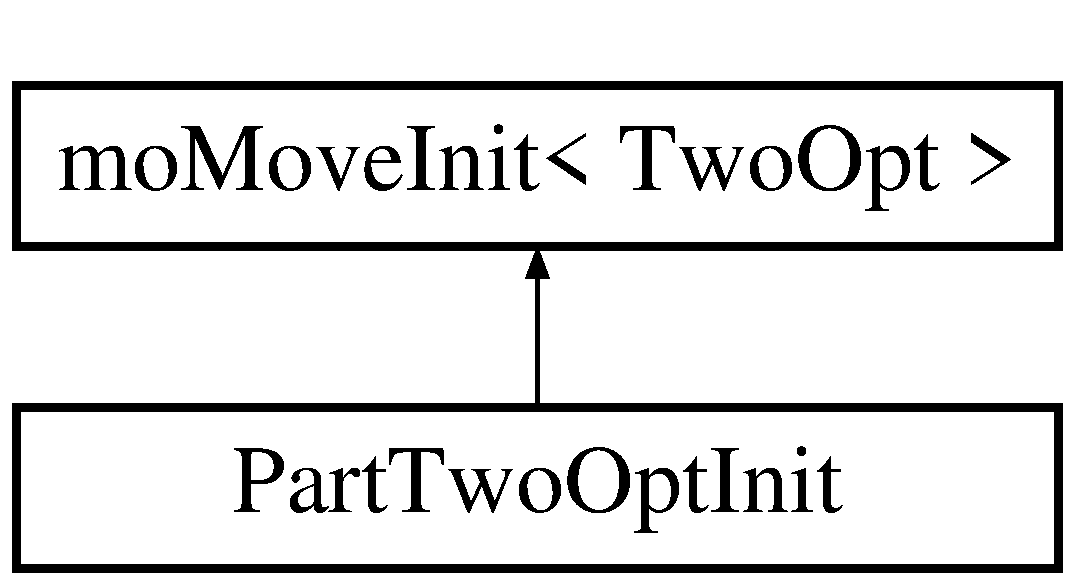
\includegraphics[height=2cm]{class_part_two_opt_init}
\end{center}
\end{figure}
\subsection*{Public Member Functions}
\begin{CompactItemize}
\item 
void {\bf operator()} ({\bf TwoOpt} \&\_\-\_\-move, const Route \&\_\-\_\-route)\label{class_part_two_opt_init_2f6190b1700ca1a12d0baaceaf75383c}

\end{CompactItemize}


\subsection{Detailed Description}
It sets the first couple of edges. 



Definition at line 20 of file part\_\-two\_\-opt\_\-init.h.

The documentation for this class was generated from the following files:\begin{CompactItemize}
\item 
part\_\-two\_\-opt\_\-init.h\item 
part\_\-two\_\-opt\_\-init.cpp\end{CompactItemize}
